\documentclass[a4paper,twoside,12pt]{book}

\usepackage[usenames,dvipsnames]{xcolor}


%% === nezbytné balíčky:
\usepackage{lmodern}
% \usepackage[T1]{fontenc}    % kódování písma
%\usepackage[IL2]{fontenc}  % kódování písma

\usepackage[utf8]{inputenc}     % vstupní znaková sada tohoto dokumentu: UTF-8
%\usepackage[cp1250]{inputenc}  % vstupní znaková sada tohoto dokumentu: Windows 1250
%\usepackage[latin2]{inputenc}  % vstupní znaková sada tohoto dokumentu: ISO Latin 2

\usepackage[czech, english]{babel} % česky psaná práce, typografická pravidla. Překládejte pomocí "latex.exe" nebo "pdflatex.exe"
%\usepackage{czech} % česky psaná práce. Překládejte pomocí "pdfCSlatex.exe" ("cslatex.exe" asi bude mít problém s balíkem geometry)

\usepackage[a4paper, hmarginratio=3:2]{geometry} % využití A4 stránky a nastavení okrajů (u vazby bude širší)

\usepackage{pdfpages} % pokud nemáte formulář "Zadání bak./dipl. práce" naskenovaný jako PDF, tak ZAKOMENTUJTE
\usepackage[hidelinks]{hyperref} % v PDF budou klikací odkazy ("hidelinks" je nebude rámovat)

%% === balíčky, které se mohou hodit:
%\usepackage{encxvlna} % postará se o spojky a předložky, které dle českých pravidel nesmí být na konci řádku. Dokumentace: http://texdoc.net/texmf-dist/doc/generic/encxvlna/encxvlna.pdf (chová se správně k "vnitřku" listings?)

\usepackage{graphicx} % balíček pro vkládání rastrových grafických souborů (PNG apod.)
%\usepackage{epsfig} % balíčky pro vkládání grafických souborů typu EPS
% \usepackage{float} % rozšířené možnosti umístění obrázků
% \restylefloat{table}
\usepackage{pifont}

%\usepackage{caption} % pro popisky obrázků, tabulek atd.

\usepackage{tabularx} % rozšířené možnosti tabulek
\usepackage{longtable}

\usepackage{tabu} % jiný balík pro rozšířené možnosti tabulek

\usepackage{listings}  % balíček vhodný pro ukázky zdrojového kódu v~textu práce/příloh. Nutno nastavit! http://ftp.cvut.cz/tex-archive/macros/latex/contrib/listings/listings.pdf
% \usepackage[autoload=true]{jlcode}
\usepackage{amsmath} % balíček pro pokročilou matematickou sazbu
\usepackage{amsfonts}
% \usepackage{color} % pro možnost barevného textu
%\usepackage{fancybox} % umožňuje pokročilé rámečkování
\usepackage{url}
\usepackage{bm}
\usepackage{hyperref}
\usepackage{threeparttable}
%\usepackage{index} % nutno použít v případě tvorby rejstříku balíčkem makeindex
%\newindex{default}{idx}{ind}{Rejstřík} % zavádí rejstřík v případě použití balíku index
% \usepackage{csquotes}
% \MakeOuterQuote{"}

% \frenchspacing % za větou bude mezislovní mezera (v anglických textech je mezera za větou delší)
\widowpenalty=1000 % "síla" zákazu vdov (= jeden řádek ze začátku odstavce na konci stránky)
\clubpenalty=1000 % "síla" zákazu sirotků (= jeden řádek/slovo z konce odstavce samostatně na začátku stránky)
\brokenpenalty=1000 % "síla" zákazu zlomu stránky za řádkem, který má na konci rozdělené slovo

\topmargin=-15mm      % horní okraj trochu menší
\textwidth=150mm      % šířka textu na stránce
\textheight=240mm     % "výška" textu na stránce


\pagenumbering{arabic} % číslování stránek arabskými číslicemi
\pagestyle{plain}      % stránky číslované dole uprostřed

\parindent=0pt % odsazení 1. řádku odstavce
\parskip=7pt   % mezera mezi odstavci

%% --- zde jsou zavedeny některé "konstanty" - některé musíte změnit! --- %%
\newcommand{\cvut}{České vysoké učení technické v~Praze}
\newcommand{\fjfi}{Fakulta jaderná a fyzikálně inženýrská}
\newcommand{\ksi}{Katedra softwarového inženýrství}
\newcommand{\km}{Katedra matematiky}
% \newcommand{\program}{Aplikace přírodních věd} % změňte, pokud máte jiný stud. program
\newcommand{\obor}{Aplikace informatiky v přírodních vědách} % změňte, pokud máte kurzívujiný obor

\newcommand{\druh}{Výzkumný úkol} % nebo "Diplomová práce"
\newcommand{\woman}{a} % pokud jste ŽENA, ZMĚŇTE na: ...{\woman}{a} (je to do Prohlášení)

\newcommand{\logoCVUT}{
\includegraphics{symbol_cvut_konturova_verze_cb.pdf}} % logo ČVUT -- podle grafického manuálu ČVUT platného od prosince 2016. Pokud nevyhovuje PDF-verze, tak použijte jinou variantu loga: https://www.cvut.cz/logo-a-graficky-manual -> "Symbol a logo ČVUT v Praze"). Pokud chcete logo úplně vynechat, zadejte místo "\includegraphics{...}" text "\vspace{35mm}"

% přesně podle formuláře "Zadání bak./dipl. práce" VYPLŇTE:
\newcommand{\nazevczT}{Optické rozpoznávání znaků \\ na naskenovaných historických plakátech pomocí \\nejmodernějších metod}    % český název práce (přesně podle zadání!)
\newcommand{\nazevenT}{Optical Character Recognition \\on Scanned Historical Posters Using the State-of-the-Art Methods}          % anglický název práce (přesně podle zadání!)
\newcommand{\nazevcz}{Optické rozpoznávání znaků na naskenovaných \\historických plakátech pomocí nejmodernějších metod}    % český název práce (přesně podle zadání!)
\newcommand{\nazeven}{Optical Character Recognition on Scanned Historical Posters Using the State-of-the-Art Methods}          % anglický název práce (přesně podle zadání!)
\newcommand{\autor}{Anna Gruberová}   % vyplňte své jméno a příjmení (s akademickým titulem, máte-li jej)
\newcommand{\vedouci}{Ing. Adam Novozámský, Ph.D.} % vyplňte jméno a příjmení vedoucího práce, včetně titulů, např.: Doc. Ing. Ivo Malý, Ph.D.
\newcommand{\pracovisteVed}{Computer Vision Lab, Institute of Visual Computing \& Human-Centered Technology, TU Wien - Faculty of Informatics} % ZMĚŇTE, pokud vedoucí Vaší práce není z KSI
\newcommand{\konzultant}{--} % POKUD MÁTE určeného konzultanta, NAPIŠTE jeho jméno a příjmení
\newcommand{\pracovisteKonz}{--} % POKUD MÁTE konzultanta, NAPIŠTE jeho pracoviště

% podle skutečnosti VYPLŇTE:
\newcommand{\rok}{2022}  % rok odevzdání práce (jen rok odevzdání, nikoli celý akademický rok!)
\newcommand{\kde}{Praze} % studenti z Děčína ZMĚNÍ na: "Děčíně" (doplní se k "prohlášení")

\newcommand{\klicova}{Optické rozpoznávání znaků, rozpoznávání textu, automatizace}   % zde NAPIŠTE česky max. 5 klíčových slov
\newcommand{\keyword}{Optical Character Recognition, Text Recognition, Automation}       % zde NAPIŠTE anglicky max. 5 klíčových slov (přeložte z češtiny)
\newcommand{\abstrCZ}{Optické rozpoznávání znaků z obrazových dat je žádanou úlohou v dnešním světě, jelikož pro člověka je již nemožné bez automatizace zpracovat velké množství obrazových dat. Vídeňská knihovna vlastní nad 350 tisíc digitalizovaných historických plakátů, z nichž je třeba extrahovat zobrazený text. Cílem této práce je zmapovat vybrané existující metody rozpoznávání textu a porovnat je na základě testů na vybraných datasetech.}


% zde NAPIŠTE abstrakt v češtině (cca 7 vět, min. 80 slov)
\newcommand{\abstrEN}{Optical character recognition from image data is a demanding task in today's world, because it is already impossible for humans to process a large amount of image data without automation. The Vienna Library owns over 350,000 digitized historical posters, from which the displayed text must be extracted. The aim of this work is to map selected existing text recognition methods and compare them based on tests on selected datasets.} % zde NAPIŠTE abstrakt v angličtině

\newcommand{\prohlaseni}{Prohlašuji, že jsem svou bakalářskou práci vypracoval\woman{} samostatně a použil\woman{} jsem pouze podklady (literaturu, projekty, SW atd.) uvedené v přiloženém seznamu.} % text prohlášení můžete mírně upravit :-)

\newcommand{\podekovani}{.} % NAPIŠTE poděkování, např. svému vedoucímu:
% Děkuji Ing. Eleonoře Krtečkové, Ph.D. za vedení mé bakalářské práce a za podnětné návrhy, které ji obohatily.
% NEBO:
% Děkuji vedoucímu práce doc. Pafnutijovi Snědldítětikaši, Ph.D. za neocenitelné rady a pomoc při tvorbě bakalářské práce.

\newcommand{\ti}{\textit} % zkrácený příkaz pro kurzívu
\newcommand{\tb}{\textbf} % zkrácený příkaz pro tučné písmo
\newcommand{\tn}{\texttt} % zkrácený příkaz pro neproporcionalni písmo

% Vzhled kodu - lstlistings - python
\definecolor{codegreen}{rgb}{0,0.6,0}
\definecolor{codegray}{rgb}{0.5,0.5,0.5}
\definecolor{framegray}{rgb}{0.8,0.8,0.8}
\definecolor{codepurple}{rgb}{0.58,0,0.82}
\definecolor{backcolour}{rgb}{0.95,0.95,0.92}

\lstdefinestyle{mystyle}{
    language=Python,
    frame=single,
    rulecolor=\color{framegray},
    commentstyle=\color{codegreen},
    keywordstyle=\color{magenta}\bfseries,     numberstyle=\tiny\color{codegray},
    stringstyle=\color{codepurple},
    basicstyle=\ttfamily\footnotesize,
    breakatwhitespace=false,         
    breaklines=true,                 
    captionpos=t,                    
    keepspaces=true,                 
    numbers=left,                    
    numbersep=5pt,                  
    showspaces=false,                
    showstringspaces=false,
    showtabs=false,                  
    tabsize=2
}
\lstset{style=mystyle}

\renewcommand{\lstlistingname}{Function}

%-----------------------------------------------

\newenvironment{repl}
{\fontfamily{cmvtt}\selectfont \begin{mdframed}

}{\end{mdframed}}

\usepackage[linewidth=1pt]{mdframed}


\newcolumntype{L}{>{\centering\arraybackslash}m{2cm}}
\newcolumntype{N}{>{\centering\arraybackslash}m{1.7cm}}
\newcolumntype{M}{>{\centering\arraybackslash}m{1.6cm}}
\newcolumntype{K}{>{\centering\arraybackslash}m{1.5cm}}
\newcolumntype{S}{>{\centering\arraybackslash}m{1cm}}
\renewcommand{\arraystretch}{1.3}

\newcommand{\cmark}{\textcolor{green!80!black}{\ding{51}}}
\newcommand{\xmark}{\textcolor{red}{\ding{55}}}





% todo notes
\usepackage[colorinlistoftodos]{todonotes}

\begin{document}
%%%%%%%%%%%% TITULNÍ STRANA -- na následujících cca 30 řádků NESAHEJTE!!!  Generuje se AUTOMATICKY %%%%%%%%%%%%
\thispagestyle{empty}

\begin{center}
	{\LARGE
		\cvut\par
		\fjfi
	}
    \vspace{10mm}

    \begin{tabular}{c}
		\tb{\ksi} \\[3pt]
		\tb{Obor: \obor}\\
    \end{tabular}

   \vspace{10mm} \logoCVUT \vspace{15mm}

   {\huge \tb{\nazevczT}\par}
   \vspace{5mm}
   {\huge \tb{\nazevenT}\par}

   \vspace{15mm}
   {\Large \MakeUppercase{\druh}}

   \vfill
   {\large
    \begin{tabular}{ll}
    Vypracoval: & \autor\\
    Vedoucí práce: & \vedouci\\
    Rok: & \rok
    \end{tabular}
   }
\end{center}

\clearpage{\pagestyle{empty}\cleardoublepage} % prázdná stránka za tou "titulní", bez čísla

%%%%%%%%%%%% ZADÁNÍ PRÁCE %%%%%%%%%%%%
% Zadání (podepsané děkanem!) musíte NASKENOVAT. Ideálně jako 2stránkové PDF (soubor "zadani_cele.pdf").
% Před svázáním to v jednom výtisku VYMĚNÍTE ZA ORIGINÁLNÍ ZADÁNÍ (podepsané děkanem fakulty)!
\newpage  % SEM NESAHEJTE!
\thispagestyle{empty} % SEM NESAHEJTE!

%% zde podle toho, jak jste zadání naskenovali, VYBERTE variantu A, B nebo C:
%
% --- varianta A: zadání naskenované jako 2stránkové PDF:
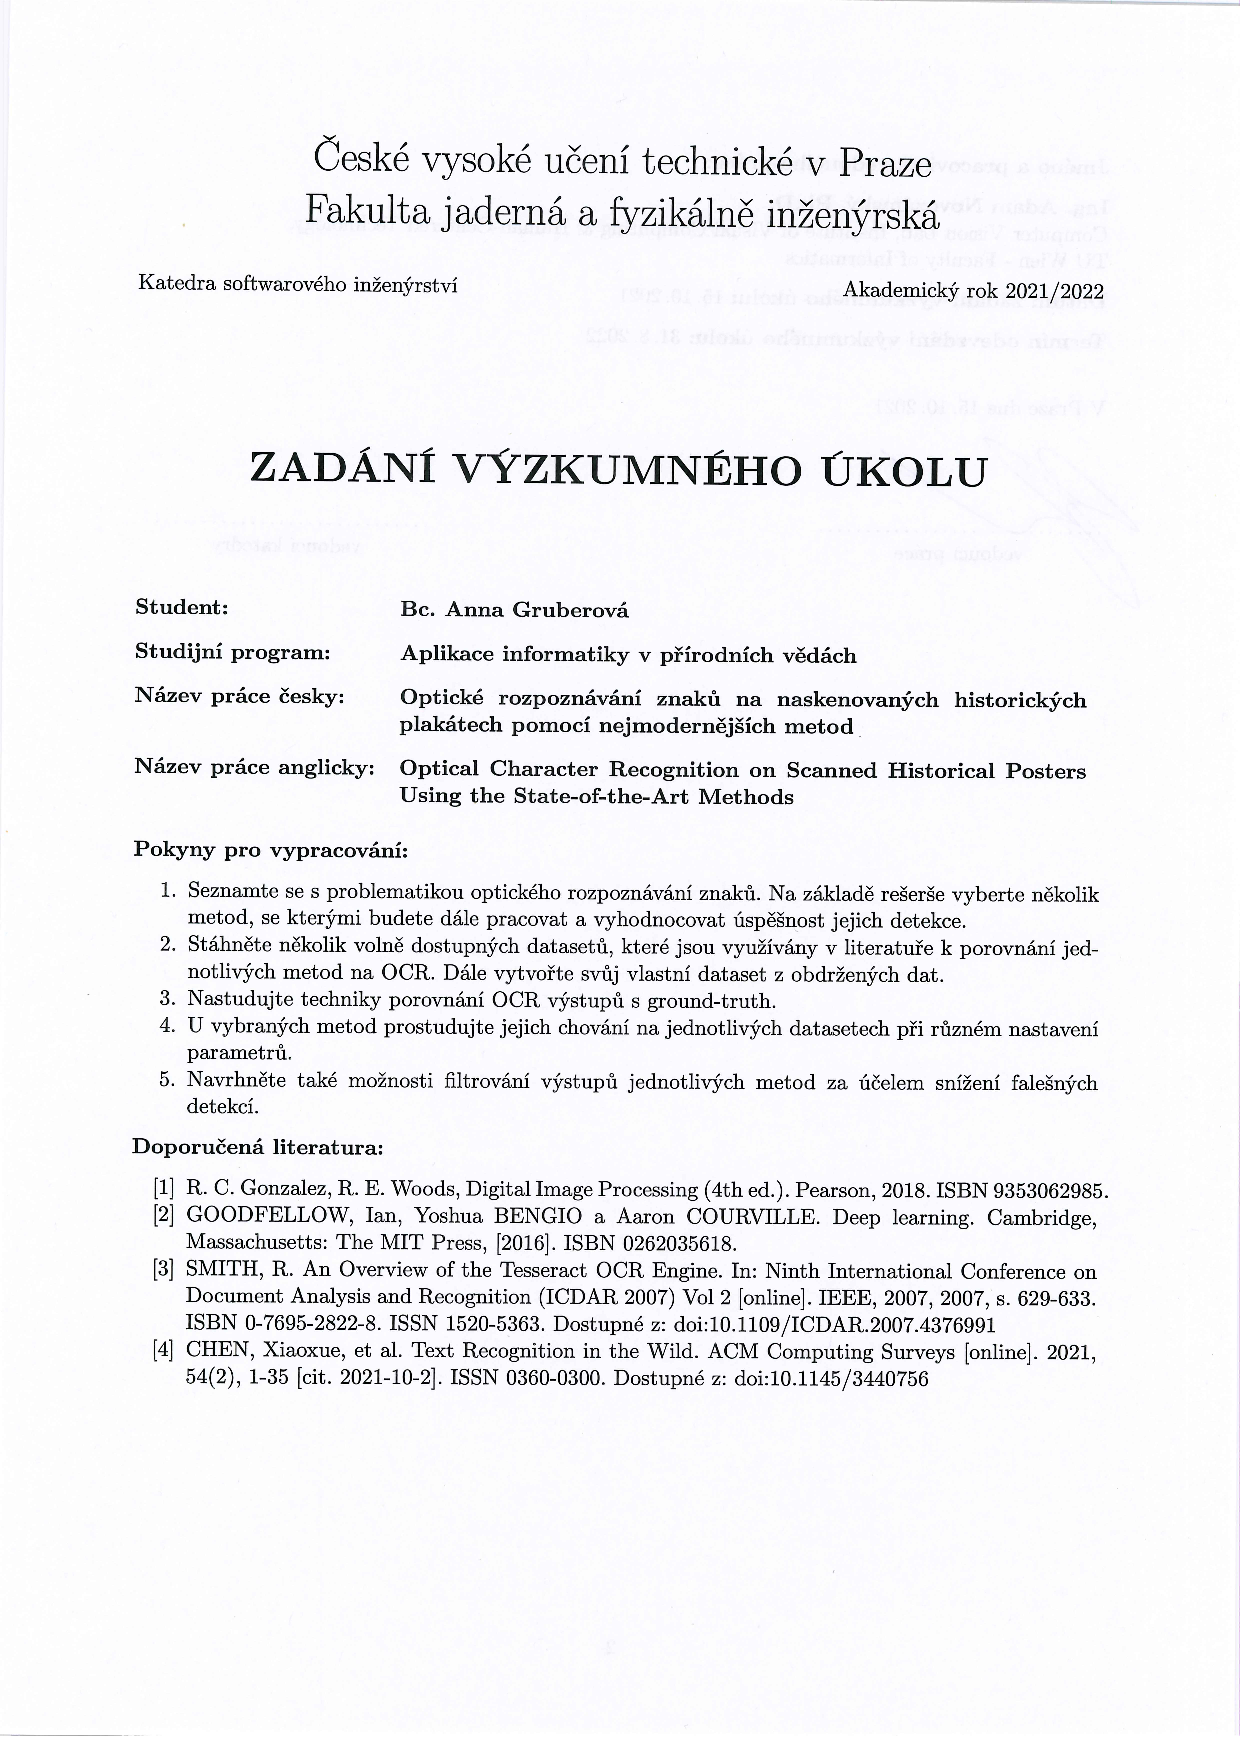
\includepdf[pages={1,2}]{zadani.pdf} % NAHRAĎTE správným souborem!!!!DOPLNIT
%
%% --- varianta B: zadání naskenované jako jednotlivé stránky:
%\includepdf[pages={1}]{zadani1.pdf} % 1. strana zadání v PDF
%\includepdf[pages={1}]{zadani2.pdf} % 2. strana zadání v PDF
%
%% --- varianta C: zadání naskenované jako 2 samostatné obrázky:
%% 1. strana zadání
%\begin{center}
%     \includegraphics[width=1\textwidth]{zadani1.jpg}
%\end{center}
%% 2. strana zadání
%\newpage  % SEM NESAHEJTE!
%\thispagestyle{empty} % SEM NESAHEJTE!
%\begin{center}
%     \includegraphics[width=1\textwidth]{zadani2.jpg}zada
%\end{center}


%%%%%%%%%%%% Prohlášení -- SEM NESAHEJTE! Generuje se automaticky z výše nastavených maker \kde{} a \prohlaseni{}. %%%%%%%%%%%%
\newpage % SEM NESAHEJTE!
\thispagestyle{empty}  % SEM NESAHEJTE!

~ % SEM NESAHEJTE!
\vfill % prázdné místo. SEM NESAHEJTE!

\tb{Prohlášení} % SEM NESAHEJTE!

\vspace{1em} % vertikální mezera. SEM NESAHEJTE!
\prohlaseni

\vspace{2em}  % SEM NESAHEJTE!
\hspace{-0.5em}\begin{tabularx}{\textwidth}{X c}  % SEM NESAHEJTE!
V \kde\ dne .................... &........................................ \\	% SEM NESAHEJTE!
	& \autor
\end{tabularx}	% SEM NESAHEJTE!


%%%%%%%%%%%% Poděkování  %%%%%%%%%%%%
\newpage
\thispagestyle{empty}

~
\vfill % prázdné místo


% -- následující kus kódu (do "%%%%%%%%%%%% ABSTRAKT") můžete odstranit, pokud nechcete psát poděkování:
\tb{Poděkování}

\vspace{1em} % vertikální mezera
\podekovani
\begin{flushright}
\autor
\end{flushright}  % <------- tady končí stránka s poděkováním


%%%%%%%%%%%% ABSTRAKT atp. Je generován AUTOMATICKY podle maker nastavených na začátku souboru) %%%%%%%%%%%%
\newpage   % SEM NESAHEJTE!
\thispagestyle{empty}   % SEM NESAHEJTE!

% příprava:    (na následujících 8 řádků NESAHEJTE!)
\newbox\odstavecbox
\newlength\vyskaodstavce
\newcommand\odstavec[2]{%
    \setbox\odstavecbox=\hbox{%
         \parbox[t]{#1}{#2\vrule width 0pt depth 4pt}}%
    \global\vyskaodstavce=\dp\odstavecbox
    \box\odstavecbox}
\newcommand{\delka}{115mm} % šířka textů ve 2. sloupci tabulky

% použití přípravy:    % dovnitř "tabular" vůbec NESAHEJTE!
\begin{tabular}{ll}
  {\em Název práce:} & ~ \\
  \multicolumn{2}{l}{\bf \nazevcz} \\[1em]
  {\em Autor:} & \autor \\[1em]
  % {\em Studijní program:} & \program \\
  {\em Obor:} & \obor \\
  {\em Druh práce:} & \druh \\[1em]
  {\em Vedoucí práce:} & \odstavec{\delka}{\vedouci\\ \pracovisteVed} \\
  {\em Konzultant:} & -- %\odstavec{\delka}{\konzultant \\ \pracovisteKonz}  % VYMAŽTE text "-- %" v případě, že jste neměli konzultanta
 \\[1em]
  \multicolumn{2}{l}{\odstavec{\textwidth}{{\em Abstrakt:} ~ \abstrCZ  }} \\[1em]
  {\em Klíčová slova:} & \odstavec{\delka}{\klicova} \\[2em]

  {\em Title:} & ~\\
  \multicolumn{2}{l}{\bf \nazeven}\\[1em]
  {\em Author:} & \autor \\[1em]
  \multicolumn{2}{l}{\odstavec{\textwidth}{{\em Abstract:} ~ \abstrEN  }} \\[1em]
  {\em Key words:} & \odstavec{\delka}{\keyword}
\end{tabular}



%%%%%%%%%%%% Obsah práce ... je generován AUTOMATICKY %%%%%%%%%%%%
\newpage  % SEM NESAHEJTE!
\parskip=0pt
\tableofcontents % SEM NESAHEJTE!
\parskip=7pt
\newpage % SEM NESAHEJTE!


%--------------------------------------------------------
%|         Zde začíná SAMOTNÁ PRÁCE (text)              |
%--------------------------------------------------------

% \chapter*{Úvod} % SEM NESAHEJTE!
% \addcontentsline{toc}{chapter}{Úvod} % SEM NESAHEJTE!
%
%


\begin{itemize}
    \item What is OCR 
    \item Datasets (types(synthetic, photos, scaned documents),problems(languages, noise, nonhorizontal text))
    \item Text detection
    \begin{itemize}
        \item Description
        \item Methods (CRAFT)
    \end{itemize}
    \item Text recognition
    \begin{itemize}
        \item Description
        \item Methods 
    \end{itemize}
    \item End-to-end systems (Annotating tool)
    \begin{itemize}
        \item[] Reading scanned documents
        \item EasyOCR
        \item keras-ocr
        \item Tesseract (PyTesseract)
        \item (Google Cloud Vision free) paid
        \item (AWS Recognition) paid 
        \item (Kili) paid
    \end{itemize}
    \item Results evaluation
    \begin{itemize}
        \item Comparison of output and ground-truth
        \item 
    \end{itemize}
    \item Testing methods on free datasets
    \item[] Description of datasets
    \item Using methods on historical posters    
    \item[] Description of dataset

\end{itemize}


\section{Scene text detection}

\section*{Methods}
\subsection{CRAFT}

CRAFT is framework for scene text detection.

\section{End-to-end systems}

\subsection{Tesseract}

Tesseract is an open source text recognition engine. It supports over 160 languages. Originally Tesseract was created by Hewlett-Packard in late 1980s, from 2006 it is developed and maintained by Google. As it does not have a built-in GUI direct use is via command line. However, there exist a significant number of GUIs for Linux, Windows, Mac for computer usage and also for Android and iOS to use on mobile phones and few online OCR services. Another way how to use the engine is via libraries for computer languages, namely for example they exist for Java called tess4j, Python called PyTesseract, R, Ruby and others. \cite{tesseract1}

Tesseract is mainly used as tool for recognizing documents (with both computer font text or hadwritten text). Best results are obtained on preprocessed images. The preprocessing includes noise reduction, horizontal alignment of text, elimination of dark borders around text region, conversion to binary black and white picture and other adjustments depending on the nature of the picture. Thus when used on scene text images it gives generally worse results than other OCR softwares. 

Computarions with Tesseract are supported for GPU and also CPU. Tesseract uses for recognition Long Short Term Memory (LSTM) model (kind of RNN).

\subsection{EasyOCR}

EasyOCR is a product of Jaded AI for both image text detection and recognition. it supports over 80 languages and various scripts such as Latin, Chinese, Arabic etc. The company offers software with web interface for free and also prepaid version which enables usage of a new model for custom data. However, in addition to the web interface, the company also created a python package under the same name.\cite{easyocr1}

The idea of EasyOCR package is to provide an easy-to-use tool where one can plug-in already created state-of-art models and use them for annotating. Pipeline of EasyOCR behavior is shown in the image \ref*{img:easyocrPipeline}. As it can be seen in this image, default detection model is CRAFT and for recognition is used CRNN (Convolutional Recurrent Neural Network) which model is composed of following components: feature extraction (Resnet is used) and VGG (Convolutional Neural Network), sequence labeling (LSTM is used) and decoding (CTC is used).\cite{easyocr2}

EasyOCR package by default computes annotation on GPU, however there is a possibility for CPU computations (provided that the selected model supports it). 

\begin{figure}[hbtp]
    \centering
    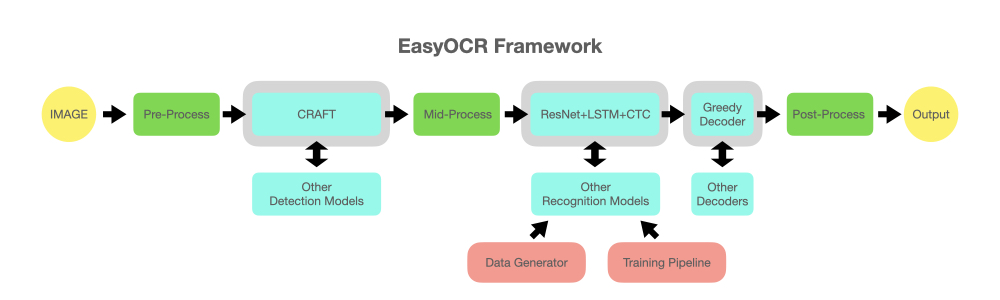
\includegraphics[scale=0.4]{obrazky/easyocr_framework.jpeg}
    \caption{Diagram of EasyOCR pipeline. Grey slots are placeholders for models. The mentioned models are the ones used as default. \cite{easyocr2}}
    \label{img:easyocrPipeline}
\end{figure}

\subsection{Keras-ocr}

keras-ocr is a python library used for detecting and recognizing text in images created by Fausto Morales. It works with variety of languages and with different writing scripts. It allows computing on CPU as well as on GPU.  It unites the CRAFT text detection model\footnote{hereinafter referred to as CRAFT} and an implementation in Keras python library of CRNN for recognizing text\footnote{hereinafter referred to as CRNN}, worth mentioning this is a different implementation of CRNN than in EasyOCR.\cite{keras-ocr1}

On the official website\footnote{\url{https://pypi.org/project/keras-ocr/}} of the package there is a comparison of this method with two other OCR APIs -- Google Cloud Vision and AWS Rekognition. Their performance was tested on 1,000 images from the COCO-Text validation set using a basic pretrained model of each method. None of the investigated methods Michalovice, 293 01 Mlada Boleslavperformed poorly; however, AWS Rekognition had the worst precision and recall results. Google's method and keras-ocr has similar results. It is important to mention that no tuning parameters were used in any of these methods. Another candidate for comparison was Tesseract but it performed on very badly on given data, most likely due to the fact that Tesseract is suitable for scanned documents rather than for photos of real life scenery and objects with text. \cite{keras-ocr1}

CRAFT already provides a pretrained model which can be used directly without modification for text detection or it is used as initial model for training a new model on new data. This model was trained on three datasets (SynthText, IC13, IC17) and supports English and multi language text detection. \cite{craft1}
Similarly for recognition, CRNN also has a pretrained model  This model was trained on the synthetic word dataset which consists of 9 million images with vocabulary of 90K English words. \cite{synth}
To use these models in the keras-ocr library one either doesn't specify anything and use the defaults, or pass the value \texttt{clovaai-general} for the CRAFT pretrained model or \texttt{kurapan} for the CRNN model.

Keras-ocr offers preprocessing for four public datasets though any text image dataset can be examined using this tool. These four datasets are: BornDigital dataset, COCO-Text dataset, ICDAR 2013 dataset, ICDAR 2019 dataset (only Latin-only scripts).\cite{keras-ocrDocu}



% \chapter*{Závěr} % SEM NESAHEJTE!
% \addcontentsline{toc}{chapter}{Závěr} % SEM NESAHEJTE!
%



%%%%%%%%%%%% SEZNAM POUŽITÝCH ZDROJŮ (LITERATURA) %%%%%%%%%%%%
\clearpage  % SEM NESAHEJTE!
\addcontentsline{toc}{chapter}{Literatura} % SEM NESAHEJTE!

% \input{tex/bibliografie1.tex}
% \bibliographystyle{unsrt}
% \bibliography{bibliografie}


%%%%%%%%%%%% PŘÍLOHY PRÁCE %%%%%%%%%%%%
\newpage % SEM NESAHEJTE!
\addcontentsline{toc}{chapter}{Přílohy} % SEM NESAHEJTE!
\appendix % SEM NESAHEJTE!


%%%%%%%%%%%% Příloha A (tj. 1. kapitola v rámci příloh) %%%%%%%%%%%%

% \chapter{Obsah přiloženého CD}
%

%
% \input{priloha_A.tex} % text vkládán ze souboru, kde je i příkaz \chapter{...}


\end{document} % SEM NESAHEJTE! Konec.
